


\documentclass[12pt]{extarticle}

\usepackage{summary-intro}


\usepackage{tikz}
\usepackage{pgfplots}
\usetikzlibrary{snakes}
\usetikzlibrary{lindenmayersystems}
\usetikzlibrary{arrows,petri,topaths}
\usetikzlibrary{plotmarks}
\usepackage{tkz-berge}
\usepackage[position=top]{subfig}



\begin{document}



\sumintro{The Banach-Tarski Theorem}{Spring 2021}










\section{The Theorem}

\begin{description}
\item[Banach-Tarski Theorem]
It is possible to decompose a ball into a finite number of pieces and
reassemble the pieces (without changing their size or shape) so as to
get two balls, each of the same size as the original.

\end{description}




\subsection{Warm-Up Case 1: A Line}\label{warm-up-case-1-a-line}


\begin{quote}
It is possible to decompose $[0,\infty) - \{1\}$ into two distinct parts, and reassemble the parts (without changing their size or shape) so as to get back $[0,\infty)$. 


\end{quote}

\vspace{2mm}
\begin{center}
\begin{tikzpicture}
\draw[thin] (-1,0) -- (-0.03,0); % straight line left
\draw (0,0) circle [radius=0.035cm]; %circle
\draw[thin] (0.03,0) -- (5.5,0); % straight line right
\draw[dotted] (5.5,0) -- (6,0); % dotted right
\node at (0,-0.4) {\tiny $1$}; % 1 label on straight


\end{tikzpicture}
\end{center}


\begin{itemize}

\item Decompose $[0,\infty) - \{1\}$ into: $(i)$ $\set{2,3,4,\dots}$ and $(ii)$ everything else.

\item Translate $\set{2,3,4,\dots}$ one unit to the left.
\end{itemize}






\subsection{Warm-Up Case 2: A Circle}\label{warm-up-case-2-a-circle}


\begin{quote}
It is possible to decompose $S^1 - \{p\}$ into two distinct parts, and reassemble the parts (without changing their size or shape) so as to get back $S^1$. 


\end{quote}





\begin{center}
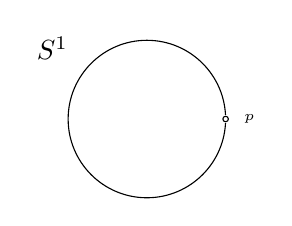
\begin{tikzpicture}
\draw (0,0) circle [radius=1cm]; %circle
\draw[line width=0.1cm, white] (0:0.9) -- (0:1.1); % gap on circle
\draw (1,0) circle [radius=0.035cm]; %circle
\node at (1.3,0) {\tiny $p$}; % 0 label on circle
\node at (-1.2,.9) { $S^1$}; % 0 label on circle

\end{tikzpicture}
\end{center}

\vspace{4mm}

\begin{itemize}

\item Decompose $S^1 - \{p\}$ into: $(i)$ $B$ and $(ii)$ everything else.

\item Rotate $B$ one unit counter-clockwise.
\end{itemize}

%\vspace{2mm}
$$B = \set{x \in S^1 : \text{$x$ is $n$ units clockwise from $p$ } (n \in \mathbb{Z}^+)}$$


\begin{center}
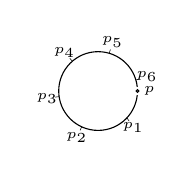
\begin{tikzpicture}[scale=0.50]
\draw (0,0) circle [radius=1cm]; %circle
\draw[line width=0.1cm, white] (0:0.9) -- (0:1.1); % 0 gap on circle
\draw (1,0) circle [radius=0.035cm]; %circle
\node at (1.3,0) {\tiny $p$}; % p label 
\draw[very thin] (0.7336545585,-0.6795226184) -- (0.787684789,-0.7636697168); % p1 tick
\node at (0.8957452502,-0.9319639138) {\tiny $p_1$}; % p1 label 
\draw[very thin] (-0.4161468365,-0.9092974268) -- (-0.4577615202,-1.00022717); % p2 tick
\node at (-0.5409908875,-1.182086655) {\tiny $p_2$}; % p2 label 
\draw[very thin] (-0.9899924966,-0.1411200081) -- (-1.088991746,-0.1552320089); % p3 tick
\node at (-1.286990246,-0.1834560105) {\tiny $p_3$}; % p3 label 
\draw[very thin] (-0.6536436209,0.7568024953) -- (-0.7190079829,0.8324827448); % p4 tick
\node at (-0.8497367071,0.9838432439) {\tiny $p_4$}; % p4 label 
\draw[very thin] (0.2836621855,0.9589242747) -- (0.312028404,1.054816702); % p5 tick
\node at (0.3687608411,1.246601557) {\tiny $p_5$}; % p5 label 
\draw[very thin] (0.9601702867,0.2794154982) -- (1.056187315,0.307357048); % p6 tick
\node at (1.248221373,0.3632401477) {\tiny $p_6$}; % p6 label 
%\draw[very thin] (0.7539022543,-0.6569865987) -- (0.8292924798,-0.7226852586); % p7 tick
%\node at (0.9800729306,-0.8540825783) {\tiny $p_7$}; % p7 label 
\end{tikzpicture}\\
{\footnotesize The first six members of $B$.}
\end{center}


\subsection{Warm-Up Case 3: The Cayley Graph}\label{the-cayley-graph}

\begin{quote}
It is possible to decompose (the set of endpoints of) the Cayley Graph\footnote{A {Cayley Path} is a {finite} sequence of steps starting from $c$, where no step follows its inverse. The Cayley Graph $C$ is the set of Cayley Paths. $X^e$ is the set of endpoints of Cayley paths in $X$.} into four distinct parts, and reassemble the parts (albeit changing their size) so as to get back \emph{two copies} of the same size as the original. 


\end{quote}



\begin{center}
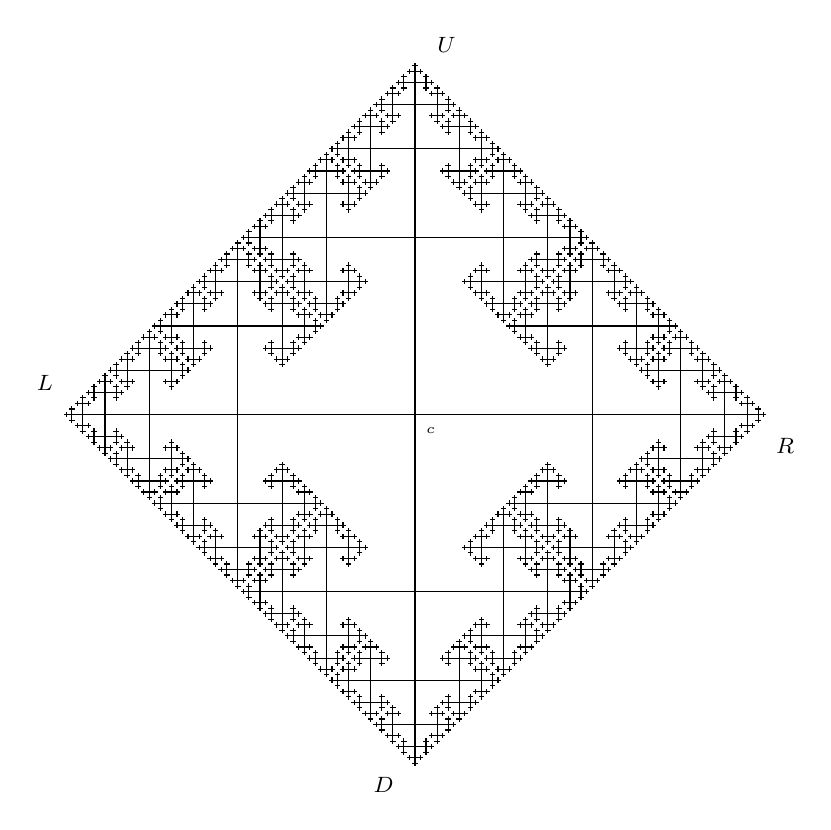
\begin{tikzpicture}
\pgfdeclarelindenmayersystem{Cayley}{
\rule{G -> [FFFFFFFFFFFFFFFFFFFFFFFFFFFFFFFFE][+FFFFFFFFFFFFFFFFFFFFFFFFFFFFFFFFE][+++FFFFFFFFFFFFFFFFFFFFFFFFFFFFFFFFE]}
\rule{E -> [FFFFFFFFFFFFFFFFD][+FFFFFFFFFFFFFFFFD][+++FFFFFFFFFFFFFFFFD]}
\rule{D -> [FFFFFFFFC][+FFFFFFFFC][+++FFFFFFFFC]}
\rule{C -> [FFFFB][+FFFFB][+++FFFFB]}
\rule{B -> [FFA][+FFA][+++FFA]}
\rule{A -> [F][+F][+++F]}
}
% Right
\draw[l-system={Cayley, step=1pt, angle=90, axiom=[FFFFFFFFFFFFFFFFFFFFFFFFFFFFFFFFFFFFFFFFFFFFFFFFFFFFFFFFFFFFFFFFG], order=6}]
lindenmayer system;
% Top
\draw[l-system={Cayley, step=1pt, angle=90, axiom=[+FFFFFFFFFFFFFFFFFFFFFFFFFFFFFFFFFFFFFFFFFFFFFFFFFFFFFFFFFFFFFFFFG], order=6}]
lindenmayer system;
% Left
\draw[l-system={Cayley, step=1pt, angle=90, axiom=[++FFFFFFFFFFFFFFFFFFFFFFFFFFFFFFFFFFFFFFFFFFFFFFFFFFFFFFFFFFFFFFFFG], order=6}]
lindenmayer system;
% Bottom
\draw[l-system={Cayley, step=1pt, angle=90, axiom=[+++FFFFFFFFFFFFFFFFFFFFFFFFFFFFFFFFFFFFFFFFFFFFFFFFFFFFFFFFFFFFFFFFG], order=6}]
lindenmayer system;
\node at (0.2,-0.2) {\tiny $c$}; % c label 
\node at (0.4,4.7) {\footnotesize $U$}; % U label 
\node at (4.7,-0.4) {\footnotesize $R$}; % R label 
\node at (-0.4,-4.7) {\footnotesize $D$}; % D label 
\node at (-4.7,0.4) {\footnotesize $L$}; % L label 

\end{tikzpicture}
\end{center}



%\vspace{4mm}

\begin{itemize}

\item Decompose $C^e$ into quadrants: $L^e, R^e, U^e, D^e$.

\item Make first copy by expanding $R^e$ and translating left to meet $L^e$.

\item Make second copy by expanding $U^e$ and translating down to meet $D^e$.
\end{itemize}





\subsection{A more abstract description of the procedure}\label{sec:bt-abstract}

\begin{quote}
\emph{Notation:} if \(X\) is a set of Cayley Paths, let \(\stackrel{\leftarrow}{X}\) be the set that results from  eliminating the first step from each of the Cayley Paths in \(X\).


\end{quote}
By the definition of Cayley Paths:
\begin{enumerate}
\item[(\(\alpha\))] \(C =  \stackrel{\leftarrow}{R} \cup \, L\)

\item[(\(\beta\))] \(C =  \stackrel{\leftarrow}{D} \cup \, U\)

\end{enumerate}
Since every Cayley Path has a unique endpoint, \((\alpha)\) and \((\beta)\) entail:
\begin{enumerate}
\item[(\(\alpha'\))] \(C^e =  \left(\stackrel{\leftarrow}{R}\right)^e \cup \, L^e\)

\item[(\(\beta'\))] \(C^e =  \left(\stackrel{\leftarrow}{D}\right)^e \cup \, U^e\)
\end{enumerate}
On our two-dimensional interoperation of the Cayley Graph, this delivers the intended result because:

\begin{enumerate}

\item  \(C^e\) is decomposed into \(U^e\), \(D^e\), \(L^e\) and \(R^e\) (ignoring the central vertex)

\item One can get from \(R^e\) to \(\left(\stackrel{\leftarrow}{R}\right)^e\), and from \(D^e\) to \(\left(\stackrel{\leftarrow}{D}\right)^e\), by performing a translation together with an expansion. (See figure~\ref{fi:dec}.)

[So our duplication requires only translations and expansions.]


\end{enumerate}






\begin{figure}
\begin{center}
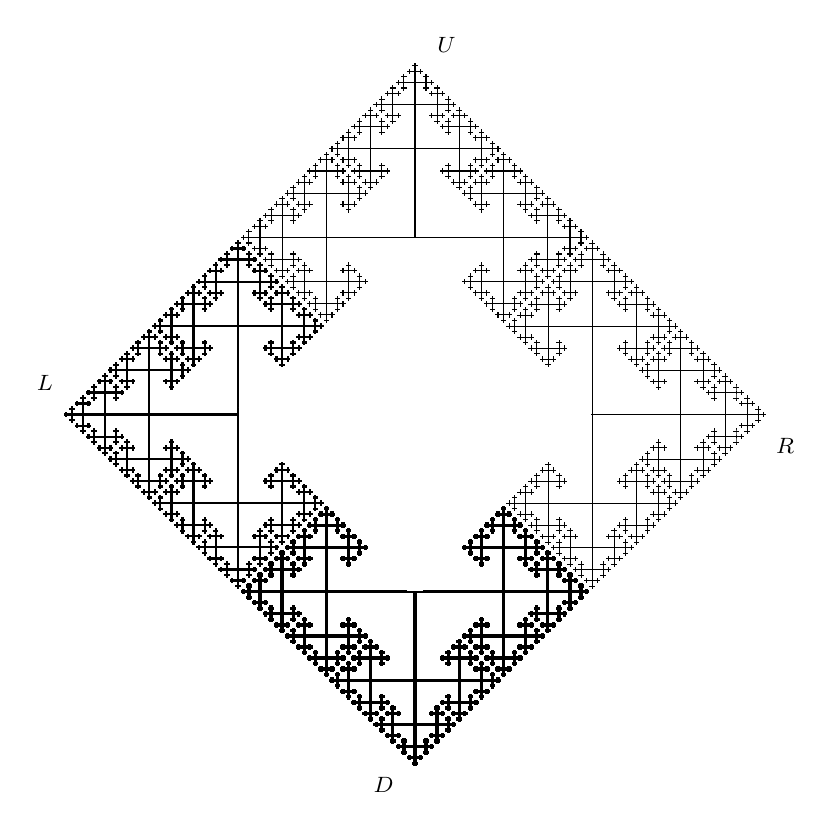
\begin{tikzpicture}
\pgfdeclarelindenmayersystem{CayleyA}{
\rule{G -> [FFFFFFFFFFFFFFFFFFFFFFFFFFFFFFFFE][+FFFFFFFFFFFFFFFFFFFFFFFFFFFFFFFFE][+++FFFFFFFFFFFFFFFFFFFFFFFFFFFFFFFFE]}
\rule{E -> [FFFFFFFFFFFFFFFFD][+FFFFFFFFFFFFFFFFD][+++FFFFFFFFFFFFFFFFD]}
\rule{D -> [FFFFFFFFC][+FFFFFFFFC][+++FFFFFFFFC]}
\rule{C -> [FFFFB][+FFFFB][+++FFFFB]}
\rule{B -> [FFA][+FFA][+++FFA]}
\rule{A -> [F][+F][+++F]}
}
% Right
\draw[very thin][l-system={CayleyA, step=1pt, angle=90, axiom=[FFFFFFFFFFFFFFFFFFFFFFFFFFFFFFFFFFFFFFFFFFFFFFFFFFFFFFFFFFFFFFFFG], order=6}]
lindenmayer system;
% Top
\draw[l-system={CayleyA, step=1pt, angle=90, axiom=[+FFFFFFFFFFFFFFFFFFFFFFFFFFFFFFFFFFFFFFFFFFFFFFFFFFFFFFFFFFFFFFFFG], order=6}]
lindenmayer system;
% Left
\draw[thick][l-system={CayleyA, step=1pt, angle=90, axiom=[++FFFFFFFFFFFFFFFFFFFFFFFFFFFFFFFFFFFFFFFFFFFFFFFFFFFFFFFFFFFFFFFFG], order=6}]
lindenmayer system;
% Bottom
\draw[very thick][l-system={CayleyA, step=1pt, angle=90, axiom=[+++FFFFFFFFFFFFFFFFFFFFFFFFFFFFFFFFFFFFFFFFFFFFFFFFFFFFFFFFFFFFFFFFG], order=6}]
lindenmayer system;
\draw[line width=0.2cm, white] (-2.24,0) -- (2.24,0); % blank line x
\draw[line width=0.2cm, white] (0,-2.24) -- (0,2.24); % blank line y
\node at (0.4,4.7) {\footnotesize $U$}; % U label 
\node at (4.7,-0.4) {\footnotesize $R$}; % R label 
\node at (-0.4,-4.7) {\footnotesize $D$}; % D label 
\node at (-4.7,0.4) {\footnotesize $L$}; % L label 
\end{tikzpicture}


\vspace{3mm}

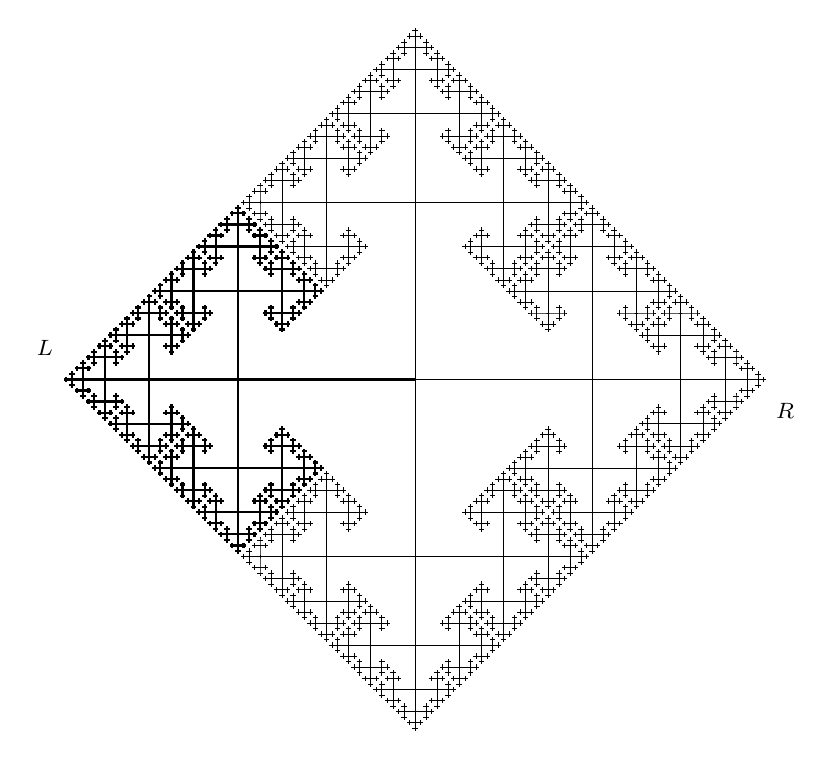
\begin{tikzpicture}
\pgfdeclarelindenmayersystem{CayleyB}{
\rule{G -> [FFFFFFFFFFFFFFFFFFFFFFFFFFFFFFFFE][+FFFFFFFFFFFFFFFFFFFFFFFFFFFFFFFFE][+++FFFFFFFFFFFFFFFFFFFFFFFFFFFFFFFFE]}
\rule{E -> [FFFFFFFFFFFFFFFFD][+FFFFFFFFFFFFFFFFD][+++FFFFFFFFFFFFFFFFD]}
\rule{D -> [FFFFFFFFC][+FFFFFFFFC][+++FFFFFFFFC]}
\rule{C -> [FFFFB][+FFFFB][+++FFFFB]}
\rule{B -> [FFA][+FFA][+++FFA]}
\rule{A -> [F][+F][+++F]}
}
% Right
\draw[very thin][l-system={CayleyB, step=1pt, angle=90, axiom=[FFFFFFFFFFFFFFFFFFFFFFFFFFFFFFFFFFFFFFFFFFFFFFFFFFFFFFFFFFFFFFFFG], order=6}]
lindenmayer system;
% Top
\draw[very thin][l-system={CayleyB, step=1pt, angle=90, axiom=[+FFFFFFFFFFFFFFFFFFFFFFFFFFFFFFFFFFFFFFFFFFFFFFFFFFFFFFFFFFFFFFFFG], order=6}]
lindenmayer system;
% Left
\draw[thick][l-system={CayleyB, step=1pt, angle=90, axiom=[++FFFFFFFFFFFFFFFFFFFFFFFFFFFFFFFFFFFFFFFFFFFFFFFFFFFFFFFFFFFFFFFFG], order=6}]
lindenmayer system;
% Bottom
\draw[very thin][l-system={CayleyB, step=1pt, angle=90, axiom=[+++FFFFFFFFFFFFFFFFFFFFFFFFFFFFFFFFFFFFFFFFFFFFFFFFFFFFFFFFFFFFFFFFG], order=6}]
lindenmayer system;
\node at (4.7,-0.4) {\footnotesize $R$}; % R label 
\node at (-4.7,0.4) {\footnotesize $L$}; % L label 
\end{tikzpicture}
\end{center}
\caption{A translation together with an expansion}
\label{fi:dec}
\end{figure}





\section{Back to the Main Event}
To prove the actual theorem, we're going to work with a \textbf{different interpretation} of the Cayley Graph, on which the graph is wrapped around the surface of a ball. 

\vspace{4mm}
\noindent
On this other interpretation, we'll have:
\begin{itemize}


\item  Different Cayley Paths have different endpoints.\footnote{Or close enough... See below!}

[So \(C^e\) is decomposed into \(U^e\), \(D^e\), \(L^e\) and \(R^e\), ignoring the center.]

\item One can get from \(R^e\) to \(\left(\stackrel{\leftarrow}{R}\right)^e\), and from \(D^e\) to \(\left(\stackrel{\leftarrow}{D}\right)^e\), by performing a \emph{rotation}. 

[So our duplication requires only rotations.]

\end{itemize}







\subsection{An external coordinate system on the ball}


\begin{itemize}

\item The \(x\)-axis runs from your right to your left through the center of the ball. 

\item The \(y\)-axis runs is orthogonal to the \(x\)-axis. It runs from the wall in front of you to the wall in behind of you, through the center of the ball.

\item The the \(z\)-axis is orthogonal to the other two. It runs from the ground to the sky, through the center of the ball. 

\end{itemize}


\subsection{A spherical interpretation of the Graph}
\begin{itemize}
\item The ``center'' of our graph is interpreted as an arbitrary point $c$ on the surface of our ball. 

\item A ``step'' is interpreted as the result of performing a \emph{rotation} on the sphere, by a certain angle $\theta$:




\begin{itemize}

\item An ``up'' rotation is a counterclockwise rotation of \(\theta\) degrees about the \(x\) axis. (When you're holding the ball in front of you, you perform this rotation by rotating the ball from bottom to top.)

\item A ``down'' rotation is a clockwise rotation of \(\theta\) degrees about the \(x\) axis. (When you're holding the ball in front of you, you perform this rotation by rotating the ball from top to bottom.)

\item A ``right'' rotation is a counterclockwise rotation of \(\theta\) degrees about the \(z\) axis. (When you're holding the ball in front of you, you perform this rotation by rotating the ball from left to right.)

\item A ``left'' rotation is a clockwise rotation of \(\theta\) degrees about the \(z\) axis. (When you're holding the ball in front of you, you perform this rotation by rotating the ball from right to left.)


\end{itemize}



\end{itemize}

\subsection{The endpoints of Cayley Paths}

\begin{itemize}

\item To each rotation \(\rho\) corresponds a function \(f_\rho\), which takes each point \(p\) on the surface of the ball to the point on the surface of the ball whose current location (relative to an external reference frame) would come to be occupied by \(p\) were rotation \(\rho\) to be performed. 

\item The ``endpoint" of Cayley Path \(\seq{\rho_1,\rho_2,\dots,\rho_n}\) is the point $$f_{\rho_1}(f_{\rho_2}(\dots f_{\rho_n}(c)\dots))$$


\end{itemize}




\subsection{Two key results}

When the rotation \(\theta\) is chosen properly,\footnote{For instance:  \(\theta = \text{arccos}(1/3) \approx 70.53^\circ\)} we get a nice result:
\begin{itemize}


\item \textbf{Result 1:} Different Cayley Paths always have different endpoints.\footnote{Annoyingly, this result holds for \emph{almost} every choice of our ``central'' point \(c\) but not quite every choice. I'll come back to this\dots}


In other words: if \(\seq{\rho_1,\rho_2,\dots,\rho_n}\) and \(\seq{\sigma_1,\sigma_2,\dots,\sigma_m}\) are distinct Cayley Paths, then \[f_{\rho_1}(f_{\rho_2}(\dots f_{\rho_n}(c)\dots)) \neq f_{\sigma_1}(f_{\sigma_2}(\dots f_{\sigma_m}(c)\dots))\] 



\item \textbf{Result 2:} One can get from \(R^e\) to \(\left(\stackrel{\leftarrow}{R}\right)^e\), and from \(D^e\) to \(\left(\stackrel{\leftarrow}{D}\right)^e\), by performing a rotation. 
\end{itemize}





\subsection{Duplicating the Surface of the Ball}

\begin{itemize}

\item Partition the surface of the ball into cells, with two points are in same cell if they are linked by a Cayley Path. 

\item Choose a ``center'' for each cell.\footnote{Rather than specifying a center for each cell, we use the Axiom of Choice to prove that a set of cell-centers exists.} 

(This delivers a partition of the surface of the ball into Cayley Graphs.)

\item Perform the duplication procedure to each Cayley Graph symultaneously.

\end{itemize}

\subsubsection{A complication}

Wait! For \(\seq{\rho_1,\rho_2,\rho_3,\dots}\) a Cayley Path:
\begin{itemize}

\item \(f_{\rho_1}(f_{\rho_2}(f_{\rho_r}(\dots)))\) is a rotation (by Euler's Theorem).


\item So \(f_{\rho_1}(f_{\rho_2}(f_{\rho_r}(\dots)))\) does not change the location of the points intersecting its axis of rotation. 

\item So whenever \(c\) is such that some such problem point is the endpoint of some Cayley Path, we will have different Cayley Paths sharing an endpoint. 
\end{itemize}

The good news:

\begin{itemize}

\item There are only countably many problem points.


\item One can deal with these points separately, by applying a sophisticated version of the trick we used in Warm-Up Case 2.


\end{itemize}


\subsection{Duplicating the Ball}

\begin{itemize}

\item Use the same procedure as before, but rather than working with points on the surface of the ball, work with the lines that connect the center of the ball with each point.

\item Wait! What about the center of the ball?
\end{itemize}


\section{A region with no volume}

Some of the Banach-Tarski pieces must be non-measurable and therefore lack definite volumes!





\end{document}






